\documentclass[11pt]{article}

\usepackage[T1]{fontenc}
\usepackage[utf8]{inputenc}
\usepackage{amsmath,amssymb,amsthm}
\usepackage{graphicx}
\usepackage[a4paper,margin=1.1in]{geometry}
\usepackage{microtype}
\usepackage{xcolor}
\usepackage[colorlinks=true,linkcolor=blue!60!black,citecolor=blue!60!black,urlcolor=blue!60!black]{hyperref}

\newtheorem{theorem}{Theorem}[section]
\newtheorem{lemma}[theorem]{Lemma}
\newtheorem{proposition}[theorem]{Proposition}
\newtheorem{corollary}[theorem]{Corollary}
\theoremstyle{remark}
\newtheorem*{remarks}{Remarks}

\newtheorem*{thmA}{Theorem A}
\newtheorem*{thmB}{Theorem B}

\newcommand{\dout}{d^{+}}
\newcommand{\din}{d^{-}}
\newcommand{\Cmain}{C_{\mathrm{main}}}
\newcommand{\inn}[1]{S(#1)}

\title{A planar triangulation with no partition into\\ two induced pseudoforests}
\author{Shaoheng Lai\thanks{Independent researcher. Email:
\texttt{laishaoheng1996@gmail.com}. See the final section for an AI-use
disclosure.}}
\date{August 18, 2026}

\begin{document}
\maketitle

\begin{abstract}
We answer a question of L.~Ploscaru (20th Eml\'ekt\'abla Workshop, 2026) in
the negative: there is a planar triangulation on $58$ vertices that admits
no orientation with $\min(\dout(v),\din(v))\le 1$ at every vertex~$v$ ---
equivalently, whose vertex set cannot be partitioned into two induced
pseudoforests. The construction substitutes three copies of a
non-Hamiltonian cubic fragment into $K_4$; the fragment is obtained by
deleting a vertex from a smallest counterexample to Tait's conjecture, the
$38$-vertex Barnette--Bos\'ak--Lederberg graph. Infeasibility follows from
an Euler-characteristic identity for the system of dual curves induced by
any candidate partition, together with a pigeonhole argument in the spirit
of Tutte's refutation of Tait's conjecture. Exhaustive SAT verification
shows that every planar triangulation on $n\le 17$ vertices does admit
such a partition, so a minimum counterexample has between $18$ and $58$
vertices.
\end{abstract}

\section{Introduction}

A \emph{pseudoforest} is a graph in which every connected component
contains at most one cycle. At the 20th Eml\'ekt\'abla Workshop (2026),
L.~Ploscaru posed the following problem \cite[p.~17]{Plo26}.

\begin{quote}
\textbf{Problem 1.} Does every planar triangulation admit an orientation
such that $\min\bigl(\dout(v),\din(v)\bigr)\le 1$ for every vertex $v$?
\end{quote}

As noted there, requiring $\min=0$ is impossible (it forces
bipartiteness), while $\min\le 2$ follows by an easy induction on a vertex
of degree at most~$5$; and the problem is equivalent to asking whether
$V(T)$ can be partitioned into two sets each inducing a pseudoforest. The
two-\emph{forest} analogue fails: planar graphs have vertex arboricity at
most $3$ \cite{CKW68}, and the bound is sharp \cite{CK69}; indeed a
triangulation has vertex arboricity at most $2$ if and only if its dual is
Hamiltonian \cite{Stein71,HS89}, so the dual of any non-Hamiltonian
$3$-connected cubic planar graph --- e.g.\ the $21$-vertex duals of the
$38$-vertex graphs of \cite{HM88} --- is a triangulation needing three
forests. Pseudoforests sit strictly between: a triangulation has $3n-6$
edges, and two induced pseudoforests can carry at most $n$ of them, so the
question is whether the remaining ${\ge}\,2n-6$ edges can always be pushed
into the bipartite cut --- tantalizingly close to the $2n-4$ maximum for
planar bipartite graphs.

We show that the answer is no.

\begin{thmA}\label{thm:A}
There is a planar triangulation $T^{*}$ on $58$ vertices whose vertex set
cannot be partitioned into two induced pseudoforests; equivalently,
$T^{*}$ has no orientation with $\min(\dout(v),\din(v))\le 1$ everywhere.
\end{thmA}

\begin{thmB}\label{thm:B}
Every planar triangulation on $n\le 17$ vertices admits such a partition.
Hence a minimum counterexample has $18\le n\le 58$ vertices.
\end{thmB}

Here and throughout, a \emph{planar triangulation} is a simple maximal
planar graph on $n\ge 4$ vertices (automatically $3$-connected); this is
the class generated by \texttt{plantri} \cite{plantri} and enumerated by
OEIS A000109.

The equivalence between the orientation and partition formulations is
recalled in Proposition~\ref{prop:equiv}. Our main tool
(Lemma~\ref{lem:rank}) converts a candidate partition into a system of
disjoint closed curves in the dual cubic graph and computes the cyclomatic
number of each monochromatic piece from the curve topology. The
counterexample then emerges from a Hamiltonicity obstruction: the curve
system would have to thread a ``through-Hamiltonian path'' across
non-Hamiltonian fragments, or pay for its failure in a currency (regions
of excess rank) that the sphere cannot supply.

\section{Partitions as curve systems}\label{sec:curves}

Throughout, $T$ is a planar triangulation embedded in the sphere $S^2$,
and $G=D(T)$ its dual: a $3$-connected simple cubic planar graph, embedded
so that each dual vertex lies in the interior of its triangle and each
dual edge crosses its primal edge exactly once and meets no other primal
edge. Whitney's theorem makes these embeddings unique up to reflection, so
the objects below are well defined.

\begin{proposition}[equivalence; stated in \cite{Plo26}]\label{prop:equiv}
A graph $G_0$ has an orientation with $\min(\dout(v),\din(v))\le 1$ for
all $v$ if and only if $V(G_0)$ can be partitioned into two sets each
inducing a pseudoforest.
\end{proposition}

\begin{proof}
($\Leftarrow$) Inside $A$, orient each pseudoforest component so that
every vertex has out-degree at most $1$: in a tree component, orient all
edges toward a root; in a unicyclic component, orient the cycle
cyclically and the remaining edges toward the cycle. Inside $B$, do the
mirror image, so that every vertex has in-degree at most $1$. Orient
every cut edge from its $B$-endpoint to its $A$-endpoint: this adds only
in-degree at $A$-vertices (which watch their out-degree) and only
out-degree at $B$-vertices (which watch their in-degree). Then
$\min(\dout,\din)\le 1$ holds at every vertex.

($\Rightarrow$) Given the orientation, put $A=\{v:\dout(v)\le 1\}$ and
$B=V\setminus A$; every $v\in B$ has $\din(v)\le 1$. Inside $A$, every
vertex has out-degree at most $1$, so each component $K$ of $G_0[A]$ has
$e(K)\le|K|$: a pseudoforest. Symmetrically for $B$.
\end{proof}

Fix now a partition $V(T)=A\cup B$. Let $X$ be the set of bichromatic
(``cut'') edges and $H$ the set of their dual edges in $G$.

\begin{lemma}[curves]\label{lem:curves}
Every vertex of $G$ has $H$-degree $0$ or $2$. Hence $H$ is a disjoint
union of simple cycles $C_1,\dots,C_k$ of $G$, drawn in $S^2$ as $k$
pairwise disjoint simple closed curves. The union of the curves meets the
primal graph exactly in one interior point of each cut edge.
\end{lemma}

\begin{proof}
A triangle with vertex colours from $\{A,B\}$ has exactly $0$ or $2$
bichromatic edges. A $2$-regular graph is a disjoint union of simple
cycles. The drawing statement is the choice of dual embedding.
\end{proof}

An $H$-cycle $C$ crosses the cut edges dual to its edges; orient $C$
arbitrarily and speak of the \emph{left} and \emph{right} endpoint of
each crossed edge.

\begin{lemma}[sides]\label{lem:sides}
Let $C$ be one of the curves, with crossed edges $e_1,\dots,e_L$ in
cyclic order. All left endpoints of the $e_j$ lie in one monochromatic
component $K_{\mathrm{left}}(C)$, all right endpoints in one
monochromatic component $K_{\mathrm{right}}(C)$, and these two components
have different colours (in particular
$K_{\mathrm{left}}(C)\ne K_{\mathrm{right}}(C)$).
\end{lemma}

\begin{proof}
Consecutive crossed edges $e_j$, $e_{j+1}$ are the two cut edges of a
common triangle $f=xyz$, say $e_j=xy$ and $e_{j+1}=xz$, where $x$ is the
minority-colour vertex of $f$. As $C$ passes through $f$ it keeps $x$ on
one fixed side and $\{y,z\}$ on the other, and $yz$ is an uncut edge. So
consecutive left endpoints are either the same vertex or joined by an
uncut edge; hence, by induction around $C$, all left endpoints lie in one
monochromatic component, and likewise on the right. A crossed edge has
one endpoint of each colour, so the two components carry different
colours.
\end{proof}

\begin{lemma}[spheres and trees; folklore, cf.\ \cite{MT01}]
\label{lem:sphere}
$k$ pairwise disjoint simple closed curves cut $S^2$ into exactly $k+1$
open connected regions; each curve lies on the boundary of exactly $2$
regions; and the bipartite incidence graph (regions vs.\ curves) is a
tree.
\end{lemma}

\begin{proof}
Induction on $k$. For $k=0$ there is one region. A new curve $\gamma$ is
connected and disjoint from the old curves, so it lies inside one
existing region $R$. All curves here are polygonal (drawings of cycles of
a plane graph), so $\gamma$ has an annular collar inside $R$ meeting no
curve; by the Jordan curve theorem $\gamma$ splits $S^2$ into two sides,
and via the collar, $R\setminus\gamma$ has exactly two components, one on
each side, each with $\gamma$ on its boundary; no other region is
affected. Thus regions increase by one, and the incidence graph is the
old one with the node $R$ split in two and joined through the new edge
$\gamma$ (old subtrees attach to the side of $\gamma$ they lie in): it
stays a tree.
\end{proof}

We call the tree of Lemma~\ref{lem:sphere} the \emph{nesting tree}. For a
region $R$ let $b_R$ denote its number of boundary curves (its degree in
the nesting tree).

\begin{lemma}[regions are monochromatic components]\label{lem:bij}
Every monochromatic component lies in exactly one region; this map is a
bijection from monochromatic components to regions; and under it the two
regions flanking a curve $C$ contain precisely $K_{\mathrm{left}}(C)$ and
$K_{\mathrm{right}}(C)$. Consequently the combinatorial incidence
(components vs.\ curves given by Lemma~\ref{lem:sides}) coincides with
the topological nesting tree.
\end{lemma}

\begin{proof}
Primal vertices and uncut edges avoid the curves (Lemma~\ref{lem:curves}),
so a monochromatic component, being connected, lies in one region. Every
region contains a primal vertex: any point $p$ of $R$ lies in a triangle
$f$; if no curve passes through $f$, all of closed $f$ (hence a vertex)
is in $R$; if the single arc of a curve through $f$ separates it, each
side contains at least one corner of $f$. In particular the map from
components to regions is surjective. Next, consider the auxiliary
multigraph $I$ with nodes the monochromatic components and one edge per
curve $C$ joining $K_{\mathrm{left}}(C)$ to $K_{\mathrm{right}}(C)$. $I$
is connected: $T$ is connected, and traversing a cut edge $uv$ moves
between exactly the two components flanking its curve ($u$ is a left or
right endpoint of a crossed edge of that curve, so its component is
$K_{\mathrm{left}}$ or $K_{\mathrm{right}}$; same for $v$). A connected
graph with $k$ edges has at most $k+1$ nodes, so
$\#\text{components}\le k+1=\#\text{regions}$; with surjectivity this
forces $\#\text{components}=k+1$ and the map is a bijection. Then $I$ is
connected with $k+1$ nodes and $k$ edges: a tree. Finally the left
endpoints of $C$ lie locally on the left of $C$, i.e.\ in the region
flanking $C$ on that side, so $I$ maps onto the topological incidence
tree node-by-node and edge-by-edge.
\end{proof}

A dual vertex not lying on any curve (equivalently, a monochromatic
triangle of $T$) is called a \emph{stray}. For a region $R$, let $w_R$ be
the number of strays in $R$.

\begin{lemma}[region rank]\label{lem:rank}
Let $K$ be a monochromatic component and $R$ its region. Then the
cyclomatic number of $T[K]$ satisfies
\[
\mu(K)\;:=\;e(K)-|K|+1\;=\;b_R-1+w_R.
\]
\end{lemma}

\begin{proof}
The closed region $\bar R$ is the sphere minus $b_R$ open disks, so
$\chi(\bar R)=2-b_R$. We exhibit a polygonal cell decomposition of
$\bar R$ and count. Write $L_i$ for the number of crossings of the $i$-th
boundary curve of $R$ ($i=1,\dots,b_R$) and $L=\sum_i L_i$.

\emph{$0$-cells}: the $|K|$ primal vertices in $R$, plus the $L$ crossing
points (one per crossed edge of a boundary curve).

\emph{$1$-cells}: the $e(K)$ uncut edges inside $R$; the $L$ half-edges
(for each crossing point, the half of its cut edge from the crossing
point to its endpoint in $K$ --- exactly one endpoint of each crossed
edge lies on $R$'s side); and the $L$ curve arcs between consecutive
crossing points (each such arc lies inside a single triangle).

\emph{$2$-cells}: the $w_R$ monochromatic triangles of $R$, plus, for
each of the $L$ boundary arcs, the piece of its (bichromatic) triangle on
$R$'s side; each piece is a disk (one is bounded by the arc and two
half-edges, the other by the arc, two half-edges and one uncut edge), and
the two pieces of one triangle lie in different regions because the two
flanks of a curve are different regions (Lemma~\ref{lem:bij}).

These cells exactly cover $\bar R$: any triangle meeting $R$ either lies
in $R$ (monochromatic, all uncut, hence entirely in one region) or is
crossed by a boundary curve of $R$. Therefore
\[
\chi(\bar R)=(|K|+L)-(e(K)+L+L)+(w_R+L)=|K|-e(K)+w_R,
\]
and equating with $2-b_R$ gives $e(K)-|K|+1=b_R-1+w_R$.
\end{proof}

As a sanity check: with $k=0$ there is one region, $b=0$, and
$w=2n-4$ faces, so the formula gives $\mu=2n-5=(3n-6)-n+1$, the
cyclomatic number of $T$ itself. The identity has also been
machine-checked on every $2$-colouring of every triangulation with
$n\le 10$ ($134{,}296$ instances) and on more than $10^6$ larger
instances; see Section~\ref{sec:verif}.

\begin{corollary}[validity criterion]\label{cor:crit}
The partition $(A,B)$ is a pseudoforest $2$-partition if and only if
every region $R$ satisfies
\begin{equation}
b_R-1+w_R\;\le\;1. \tag{$\star$}\label{eq:star}
\end{equation}
If \eqref{eq:star} holds then: every region has $b_R\le 2$, i.e.\ the
nesting tree is a path; there are at most two strays; strays lie only in
regions with $b_R=1$, i.e.\ in the two end regions of the path, at most
one stray per end region; and a region containing a stray borders exactly
one curve and contains no second stray.
\end{corollary}

\begin{proof}
The criterion is Lemma~\ref{lem:rank} applied to every monochromatic
component (``every component has $\mu\le 1$''). Note first that $k\ge 1$
in any valid partition: $k=0$ means no cut edges, so one colour class is
empty and $T$ itself would have to be a pseudoforest, but
$\mu(T)=2n-5\ge 3$ for $n\ge 4$. Now if \eqref{eq:star} holds, $w\ge 0$
forces $b\le 2$ everywhere (a path), each region has $b\ge 1$, and
$w_R\le 2-b_R\le 1$ with $w_R=1$ only if $b_R=1$; a path has exactly two
ends.
\end{proof}

\section{The construction}\label{sec:constr}

Let $\Gamma$ be a Barnette--Bos\'ak--Lederberg graph: a non-Hamiltonian
$3$-connected cubic planar graph on $38$ vertices. The minimum order of
such graphs is $38$ and is attained by exactly six graphs \cite{HM88};
they arise from the work of Barnette, of Bos\'ak \cite{Bosak67}, and of
Lederberg in the mid-1960s, so $38$ is the order of the smallest
counterexamples to Tait's conjecture \cite{Tait84,Tutte46,HM88}. We use
the copy archived as House of Graphs \#954 \cite{HoG}; its
non-Hamiltonicity is also re-verified mechanically here
(Section~\ref{sec:verif}). Fix any vertex $v_0$ of $\Gamma$ and let
$F=\Gamma-v_0$, a fragment with $34$ cubic vertices and $3$ vertices of
degree $2$ (the former neighbours of $v_0$), which we call \emph{ports}.

\begin{figure}[t]
\centering
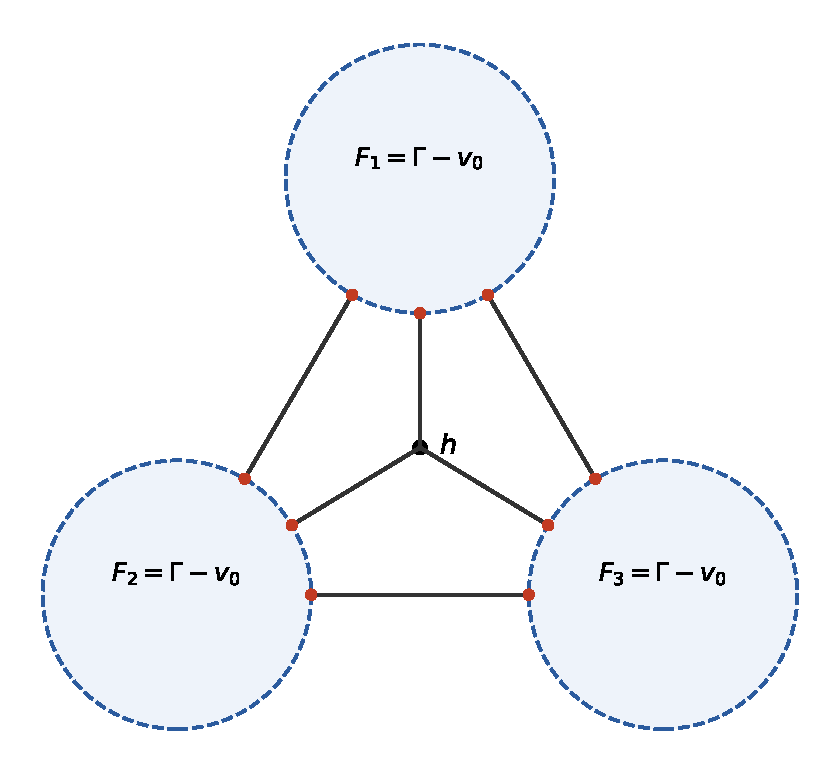
\includegraphics[width=0.62\textwidth]{fig1.pdf}
\caption{The cubic graph $G^{*}$ on $112$ vertices: a hub $h$ and three
copies $F_i$ of $F=\Gamma-v_0$, wired as $K_4$. Ports (degree-$2$
vertices of the fragments) are shown as small dots; the six connector
edges realize the $K_4$ pattern. The counterexample is
$T^{*}=D(G^{*})$.}
\label{fig:constr}
\end{figure}

\medskip
\noindent\textbf{Definition (the graph $G^{*}$).}
Take $K_4$ with vertices $h,b_1,b_2,b_3$. Substitute for each $b_i$ a
copy $F_i$ of $F$, attaching its three ports to the three $K_4$-edges at
$b_i$: one port to the edge toward $h$ (the \emph{$h$-port}) and one port
each to the edges toward the other two fragments. Keep $h$ as a single
vertex. The resulting graph $G^{*}$ is cubic on $3\cdot 37+1=112$
vertices and planar (embed each $F_i$ in a disk with its three ports on
the boundary in the rotation inherited from a planar embedding of
$\Gamma$ around $v_0$). See Figure~\ref{fig:constr}.

\begin{lemma}[substitution preserves $3$-connectivity]\label{lem:sub}
Let $G_1,G_2$ be $3$-connected cubic graphs, $u\in V(G_1)$,
$v\in V(G_2)$. Delete $u$ and $v$ and join the three former neighbours of
$u$ to the three former neighbours of $v$ by a perfect matching. The
resulting cubic graph $G$ is $3$-connected.
\end{lemma}

\begin{proof}
Write $A_1=V(G_1)-u$, $A_2=V(G_2)-v$. Let $|S|\le 2$ and suppose $G-S$ is
disconnected. Note $G_i$ minus one vertex is $2$-connected ($G_i$ is
$3$-connected), so if $S$ lies entirely in $A_1$, then $A_2$ induces a
connected subgraph of $G-S$. Any component $C$ of $(G_1-u)-S$ satisfies
$N_{G_1}(C)\subseteq S\cup\{u\}$; if $u$ is not adjacent to $C$ then
$N_{G_1}(C)\subseteq S$ is a cut of size at most $2$ in $G_1$ ($u$ lies
outside $C$, so the complement of $C\cup S$ is nonempty), impossible;
hence some vertex of $C$ was a neighbour of $u$ and retains its matching
edge into $A_2$ in $G-S$. So every component of the $A_1$-side attaches
to the connected $A_2$-side: $G-S$ is connected, a contradiction. If $S$
has one vertex on each side, then each of $(G_1-u)-s_1$ and
$(G_2-v)-s_2$ is connected ($2$-connected minus one vertex), and each
deleted vertex destroys at most one of the three matching edges, so a
matching edge survives and joins the two sides. The cases
$S\subseteq A_2$ and $|S|\le 1$ are symmetric or easier.
\end{proof}

Applying Lemma~\ref{lem:sub} three times (substituting $\Gamma$ for each
of the three chosen vertices of $K_4$; both $K_4$ and $\Gamma$ are
$3$-connected cubic) shows that $G^{*}$ is $3$-connected; this is also
verified mechanically.

\medskip
\noindent\textbf{Definition (the triangulation $T^{*}$).}
$T^{*}:=D(G^{*})$, the planar dual of $G^{*}$. Since $G^{*}$ is a simple
$3$-connected cubic planar graph on $112$ vertices with $168$ edges,
$T^{*}$ is a planar triangulation with $58$ vertices and $168$ edges
($m=3n-6$ holds), $3$-connected by Whitney. Adjacency lists and
\texttt{graph6} strings for both graphs are archived with the paper
(\texttt{data/counterexample\_58.json}).

Fix once and for all pairwise disjoint closed disks
$\Delta_1,\Delta_2,\Delta_3$ in $S^2$ (\emph{territories}) such that
$\Delta_i$ contains exactly the vertices and edges of $F_i$, with the
three attachment edges of $F_i$ crossing the boundary circle of
$\Delta_i$ transversally, once each; the complement
$P:=S^2\setminus(\Delta_1\cup\Delta_2\cup\Delta_3)$, an open connected
$3$-holed sphere, contains $h$, the six attachment edges' middle
portions, and nothing else of $G^{*}$. (Such disks exist by construction
of the embedding.)

\begin{lemma}[fragment property]\label{lem:frag}
For any two ports $a,b$ of $F$ there is no Hamiltonian path of $F$ with
endpoints $a$ and $b$.
\end{lemma}

\begin{proof}
Such a path together with the edges $av_0$ and $bv_0$ would be a
Hamiltonian cycle of $\Gamma$.
\end{proof}

\section{Proof of Theorem A}\label{sec:proof}

Suppose toward a contradiction that $T^{*}$ admits a pseudoforest
$2$-partition, and let $H=C_1\cup\dots\cup C_k$ be its curve system in
$G^{*}$ (Lemma~\ref{lem:curves}), with stray set $U$ (uncovered vertices
of $G^{*}$). By Corollary~\ref{cor:crit}: the nesting tree is a path,
$|U|\le 2$, and each stray occupies its own end region, which borders
exactly one curve and contains no second stray.

\paragraph{Step 1: the skeleton.}
Contract each territory $\Delta_i$ to a point; the six attachment edges
project to the edges of $K_4$ on $\{h,b_1,b_2,b_3\}$. For each $i$, the
number of attachment edges of $F_i$ used by $H$ is even (each curve is
closed, so it crosses the circle $\partial\Delta_i$ an even number of
times, and only along attachment edges), hence $0$ or $2$; likewise $h$
has $H$-degree $0$ or $2$. So the used attachment edges form an even
subgraph $\Sigma$ of $K_4$: either empty, or a triangle ($hb_ib_j$, or
$b_1b_2b_3$), or a $4$-cycle ($hb_ib_kb_j$). If $\Sigma$ is nonempty it
is a single cycle; each individual curve's projection is even at every
node of $K_4$, and a nonempty even subset of the edge set of a cycle is
the whole cycle, so the $H$-edges projecting onto $\Sigma$ belong to a
single curve $\Cmain$, which traverses $\Sigma$ once around. Every other
curve uses no attachment edge, hence lies inside one territory (an
\emph{internal curve} of that fragment). If $\Sigma$ is nonempty and
passes $b_i$, then $\Cmain\cap\Delta_i$ is a single path through $F_i$
between the two used ports (one visit: only two attachment edges of
$F_i$ are used) --- the \emph{arc} of $F_i$; $F_i$ is \emph{traversed}.
If $\Sigma$ avoids $b_i$ (or is empty), $F_i$ is \emph{capped}: no
attachment edge is used, so every vertex of $F_i$ is covered by internal
curves of $F_i$ or lies in $U$.

\paragraph{Step 2: inner sides.}
Let $Z$ be an internal curve of $F_i$. Of the two complementary open
disks of $Z$ in $S^2$, exactly one is disjoint from $\partial\Delta_i$;
call it the \emph{inner side} $\inn{Z}$; as $Z\subset\operatorname{int}
\Delta_i$ and $\inn{Z}$ is connected and touches $Z$, we get
$\inn{Z}\subset\operatorname{int}\Delta_i$. Consequently an internal
curve of $F_i$ is never contained in the inner side of an internal curve
of $F_j$ for $j\ne i$ (disjoint territories): curves of different
fragments never nest. Call $Z$ \emph{outermost} (in $F_i$) if $Z$ is not
contained in $\inn{Z'}$ for any other internal curve $Z'$ of $F_i$.
Every fragment possessing an internal curve possesses an outermost one
(the nesting order is a finite partial order).

\paragraph{Step 3: walk-out.}
Assume $\Sigma$ nonempty, so $\Cmain$ exists; let $R_1,R_2$ be the two
regions flanking $\Cmain$ (Lemma~\ref{lem:sphere}). We claim: \emph{the
outer flank of every outermost internal curve --- the region flanking
$Z$ on the side other than $\inn{Z}$ --- is $R_1$ or $R_2$.} Let $Z$ be
outermost in $F_i$ and $R$ its outer flank. Suppose first $F_i$ is
traversed; its arc divides $\operatorname{int}\Delta_i$ into two open
half-disks; $Z$ lies in one of them, $D'$. Any curve other than the
internal curves contained in $D'$ is disjoint from the connected set
$D'$, hence leaves all of $D'$ on one side; so any curve separating two
points of $D'$ lies in $D'$ and is an internal curve of $F_i$. Points of
$D'$ at sufficiently small distance from the arc form a connected,
curve-free collar, hence lie in one region $W$ whose closure contains
the arc. We claim $R=W$. Otherwise some internal curve $Z''$ separates,
within $D'$, a point $p$ just outside $Z$ from the collar, i.e.\
$p\in\inn{Z''}$ or $(\text{collar})\subset\inn{Z''}$. In the first case,
choosing $p$ closer to $Z$ than $\operatorname{dist}(Z,Z'')$ forces
$Z\cap\inn{Z''}\ne\emptyset$, hence $Z\subset\inn{Z''}$ ($Z$ is
connected and disjoint from $Z''$), contradicting that $Z$ is outermost.
In the second, the arc would meet the closure of $\inn{Z''}$, hence
enter $\inn{Z''}$, hence lie inside it (the arc is connected and
disjoint from $Z''$) --- impossible, since the arc reaches
$\partial\Delta_i$ while $\inn{Z''}\subset\operatorname{int}\Delta_i$.
So $R=W$, whose closure contains points of the arc $\subset\Cmain$: $R$
borders $\Cmain$, i.e.\ $R\in\{R_1,R_2\}$. If instead $F_i$ is capped,
run the same argument in $\operatorname{int}\Delta_i$ (no arc): $R$'s
closure meets $\partial\Delta_i$; but $\partial\Delta_i$ is not part of
any curve, so $R$ crosses it into the pants region $P$. Inside $P$ the
only curve portions are the (nonempty) set of arcs of $\Cmain$ along
used attachment edges (and through $h$); every component of $P$ minus
those arcs has arc points on its closure, so again $R$ borders $\Cmain$.

\begin{figure}[t]
\centering
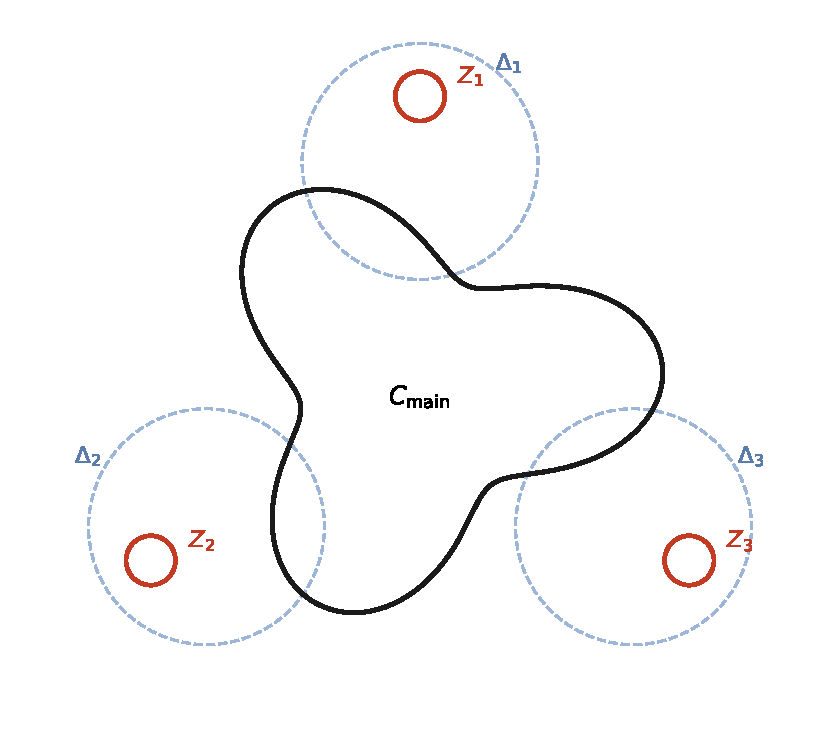
\includegraphics[width=0.58\textwidth]{fig2.pdf}
\caption{The pigeonhole. Every fragment forces a leftover cycle $Z_i$ or
an uncovered vertex (else its arc were a through-Hamiltonian path of
$F=\Gamma-v_0$, contradicting Lemma~\ref{lem:frag}); the outer flank of
each $Z_i$ borders $\Cmain$, which has only two flanks, so some region
borders at least $3$ curves, violating \eqref{eq:star}. Depicted: the
stray-free case with all three leftover cycles in the outer flank,
giving $b=4$.}
\label{fig:pigeon}
\end{figure}

\paragraph{Step 4: bookkeeping.}
Still assuming $\Sigma$ nonempty, call $F_i$ \emph{dirty} if it has at
least one internal curve, and \emph{clean} otherwise. By Step~3 each
dirty fragment nominates at least one outermost curve whose outer flank
is $R_1$ or $R_2$; distinct outermost curves are distinct boundary
curves of their flank, and $\Cmain$ also bounds $R_1$ and $R_2$. Hence,
by criterion \eqref{eq:star} ($b\le 2$):
\begin{itemize}
\item[(i)] each of $R_1,R_2$ hosts at most one outermost curve (else
$b\ge 3$); in particular at most $2$ outermost curves exist in total,
and the number of dirty fragments is at most $2$.
\item[(ii)] a capped fragment is dirty: its $37$ vertices minus at most
$2$ strays must be covered by internal curves.
\item[(iii)] a clean traversed fragment $F_i$ has
$U\cap V(F_i)\ne\emptyset$, and each such stray lies in $R_1$ or $R_2$,
which then has $b=1$. Indeed: the arc covers $V(F_i)\setminus U$
entirely, and a full cover ($U\cap V(F_i)=\emptyset$) would be a
through-Hamiltonian path, contradicting Lemma~\ref{lem:frag}. For the
placement: both half-disks of $\operatorname{int}\Delta_i$ are
curve-free ($F_i$ is clean), so each lies in a single region whose
closure contains the arc --- that region borders $\Cmain$ and is $R_1$
or $R_2$. A stray $u\in V(F_i)$ lies in one of the half-disks, so its
region is $R_1$ or $R_2$; by Corollary~\ref{cor:crit} that region then
borders exactly one curve --- so no outermost curve of any fragment
bounds it --- and hosts no second stray.
\end{itemize}

\paragraph{Step 5: case analysis, $\Sigma$ nonempty.}
Let $c\in\{0,1,2,3\}$ be the number of clean fragments (clean fragments
are traversed, by (ii)).
\begin{itemize}
\item $c=0$: three dirty fragments contradict (i).
\item $c=1$: two dirty fragments; their outermost curves must occupy
$R_1$ and $R_2$, one each, by (i). The clean fragment needs a stray
whose region is $R_1$ or $R_2$ with $b=1$ (iii) --- but both flanks now
have $b=2$. Contradiction.
\item $c=2$: one dirty fragment; the two clean fragments each need at
least one stray (iii), i.e.\ two strays $u_1\in F_i$, $u_2\in F_j$
($i\ne j$) in flanking regions with $b=1$. At least one flank hosts an
outermost curve of the dirty fragment and so has $b=2$; hence at most
one flank can host these strays, and it hosts at most one stray
(Corollary~\ref{cor:crit}). No region other than the two flanks is
available: every other region lies inside the inner side of some
internal curve, hence inside the dirty fragment's territory, which
contains no vertex of $F_i$ or $F_j$. Contradiction.
\item $c=3$: three clean fragments need three strays (iii); $|U|\le 2$.
Contradiction.
\end{itemize}

\paragraph{Step 6: degenerate skeletons.}
If $\Sigma=\emptyset$, then no attachment edge is used and $h$ has
$H$-degree $0$, so $h\in U$; all three fragments are capped, hence dirty
(ii), each with an outermost curve. The pants region $P$ now contains no
curve portion at all, so $P$ lies inside a single region $R_0$, and
(Step~3, capped case) the outer flank of every outermost curve of every
fragment crosses into $P$: all three coincide with $R_0$. Then $R_0$
borders at least $3$ curves: $b\ge 3$, contradiction.

If $\Sigma$ is nonempty but $h\in U$ ($h$ not on $\Cmain$), then
$\Sigma$ avoids $h$: $\Sigma$ is the triangle $b_1b_2b_3$, and all three
fragments are traversed. $h$ lies in $P$ minus the arcs of $\Cmain$, so
$h$'s region borders $\Cmain$ (Step~3): it is $R_1$ or $R_2$, and by
Corollary~\ref{cor:crit} it has $b=1$ and contains no second stray. The
stray budget leaves at most one stray for the fragments, so at most one
fragment is clean, i.e.\ at least $2$ are dirty. Their outermost curves
either share a flank ($b\ge 3$, contradiction) or occupy both flanks ---
and then $h$'s region has $b=2$, contradiction.

Steps 5 and 6 exhaust all configurations; the assumed partition cannot
exist. This proves Theorem~A. \qed

\begin{remarks}
(1) Only the non-Hamiltonicity of $\Gamma$ is used. The stronger
statement ``$F$ minus up to two vertices admits no port-to-port
Hamiltonian path'' is in fact false (machine check: $454$ of $1893$
deletion patterns are traversable); the argument survives because strays
cannot pay for clean traversals --- their placement is blocked by
\eqref{eq:star}, not by the fragment.
(2) Within this scheme $58$ is optimal: a fragment forcing internal
curves under all traversals must have non-Hamiltonian closure, and $38$
is the minimum order of a non-Hamiltonian $3$-connected cubic planar
graph \cite{HM88}.
(3) The construction is the classical Tutte-fragment amplification
pattern \cite{Tutte46}; the novelty is the accounting
(Lemma~\ref{lem:rank}) that converts ``not Hamiltonian'' into ``no
pseudoforest $2$-partition''.
\end{remarks}

\section{Verification}\label{sec:verif}

All claims that admit finite checks were verified mechanically; the
scripts and data are archived with the paper. An independent adversarial
review pass re-ran or re-implemented every item below from the archived
adjacency lists alone and confirmed them.

\begin{enumerate}
\item \emph{$T^{*}$ infeasible}: two independent SAT encodings --- (a)
orientation variables plus a per-vertex witness bit (witness $\Rightarrow$
pairwise at-most-one on out-edges, else on in-edges), CaDiCaL~1.9.5;
(b) colour variables plus per-edge claimed-orientation variables inside
classes, Glucose~4.2 --- both UNSAT; also UNSAT with the added
constraint ``no monochromatic face'' (the zero-stray variant). A third,
independently written encoding (review pass) reproduced UNSAT under two
further solvers.
\item \emph{Positive controls}: the same code declares the icosahedron
and random \texttt{plantri} triangulations feasible.
\item \emph{Mechanism controls}: all three fragments replaced by
traversable $3$-poles --- feasible; one BBL fragment plus two
traversable --- feasible; two BBL fragments plus one traversable ---
feasible; three BBL fragments --- infeasible. The phase transition sits
exactly where the pigeonhole predicts (three forced groups).
\item \emph{$\Gamma$ non-Hamiltonian}: verified by two further
independent methods (position-based SAT; degree constraints with lazy
subtour elimination; plus a pure backtracking search in the review
pass). Lemma~\ref{lem:frag} additionally verified directly (no
port-to-port Hamiltonian path in $F$).
\item \emph{Theorem B}: exhaustive SAT over \texttt{plantri} output for
$4\le n\le 17$. Per-order counts (matching OEIS A000109 at every
order): $1$, $1$, $2$, $5$, $14$, $50$, $233$, $1249$, $7595$, $49566$,
$339722$, $2406841$, $17490241$, $129664753$; in total $149{,}960{,}273$
triangulations, all feasible. (An earlier draft reported
$149{,}951{,}159$ due to an addition error in a running log, caught in
the review pass; the range $n=4..12$ was re-swept from scratch and the
per-order counts above are taken directly from the sweep logs.)
\item \emph{Lemmas}: the identity of Lemma~\ref{lem:rank} asserted on
more than $10^6$ (graph, partition) instances; Lemmas
\ref{lem:curves}/\ref{lem:sides}/\ref{lem:bij} and criterion
\eqref{eq:star} asserted on all valid partitions of all triangulations
with $n\le 10$ ($15{,}348$ partitions, $20{,}044$ curves) and --- in the
review pass --- on all $134{,}296$ $2$-colourings (valid or not) of all
triangulations with $n\le 10$, with zero violations.
\item \emph{Standalone verifier}: a self-contained script
(\texttt{verify\_counterexample.py}) re-derives everything from the
archived adjacency lists alone: structure checks, dual isomorphism,
non-Hamiltonicity, a positive control, and the final UNSAT.
\end{enumerate}

\section{Positive results}\label{sec:positive}

\begin{proposition}[degree-$3$ reduction]\label{prop:deg3}
If $v$ has degree $3$ in a triangulation $T$ and $T-v$ admits a valid
orientation, then so does $T$. Hence a minimum counterexample has
minimum degree at least $4$, and all stacked (Apollonian)
triangulations are feasible.
\end{proposition}

\begin{proof}
Orient each edge at $v$ in the direction harmless to its neighbour's
witness (into out-mode neighbours, out of in-mode neighbours); $v$
itself has $\dout+\din=3$, so $\min(\dout,\din)\le 1$ automatically.
\end{proof}

\begin{proposition}[dual reformulation, positive direction]
\label{prop:dual}
A triangulation $T$ is feasible if and only if $D(T)$ carries a family
of disjoint cycles whose regions all satisfy \eqref{eq:star}. In
particular any $2$-factor of $D(T)$ with at most $2$ cycles --- e.g.\ a
Hamiltonian cycle --- yields a feasible partition.
\end{proposition}

\begin{proof}
($\Rightarrow$) is Lemmas \ref{lem:curves}--\ref{lem:rank}.
($\Leftarrow$) Given such a family, $2$-colour the nodes of its nesting
tree properly (a tree is bipartite) and give the vertices inside each
region the colour of its node; then the bichromatic edges are exactly
the edges crossed by the curves, the curve system of this partition is
the given family, and Lemma~\ref{lem:rank} with \eqref{eq:star} bounds
every component's cyclomatic number by $1$. For a $2$-factor with
$k\le 2$ cycles the nesting tree is a path on at most $3$ nodes and
$w\equiv 0$, so \eqref{eq:star} holds.
\end{proof}

\paragraph{Data points.}
For every dual of a triangulation on $n=14$ vertices ($339{,}722$ cubic
graphs; over $4.8$ million non-path-nested $2$-factors), a strictly
improving single alternating-cycle flip toward a path-nested $2$-factor
exists (``no bad local minima'' of the potential
$\Phi=\#\text{leaves}-2$ of the nesting tree), and likewise for all
$n\le 13$; Theorem~A implies this landscape statement fails somewhere
in $(14,58]$.

\section{Open problems}

\begin{enumerate}
\item Determine the minimum order of a counterexample (it lies in
$[18,58]$).
\item Is deciding pseudoforest-$2$-partitionability of planar
triangulations NP-complete? The fragment scheme suggests a gadget
reduction.
\item Does every $4$-connected planar triangulation admit a pseudoforest
$2$-partition? ($T^{*}$ is full of separating triangles --- every
fragment boundary yields them.)
\item The threshold version: $\min\le 1$ fails, $\min\le 2$ holds.
Quantify the failure: how many vertices violating $\min\le 1$ can be
forced?
\end{enumerate}

\section*{Acknowledgements and AI-use disclosure}

This work was carried out in close collaboration with an AI assistant
(Anthropic Claude: models Fable~5 and Opus~5), which proposed and
executed the experimental programme, the construction, and drafts of the
proofs and text under the author's direction; a separate adversarial AI
review pass re-derived the proofs and re-implemented all machine checks
independently. All mathematical claims, references, and computational
results have been verified by the methods described in
Section~\ref{sec:verif}; the archived data and the standalone verifier
allow anyone to repeat the verification without trusting any component
of our pipeline. The AI system is not an author and bears no
responsibility for the correctness of this paper, which rests with the
human author.

\begin{thebibliography}{99}

\bibitem{Plo26} L.~Ploscaru, \emph{Orientations with almost-sources and
almost-sinks}, in: Booklet of the 20th Eml\'ekt\'abla Workshop (2026),
p.~17. \url{https://www.renyi.hu/~emlektab/Emlektab_book_2026.pdf}

\bibitem{CKW68} G.~Chartrand, H.~V.~Kronk, C.~E.~Wall, \emph{The
point-arboricity of a graph}, Israel J. Math. \textbf{6} (1968),
169--175.

\bibitem{CK69} G.~Chartrand, H.~V.~Kronk, \emph{The point-arboricity of
planar graphs}, J. London Math. Soc. \textbf{44} (1969), 612--616.

\bibitem{RW08} A.~Raspaud, W.~Wang, \emph{On the vertex-arboricity of
planar graphs}, European J. Combin. \textbf{29} (2008), 1064--1075.

\bibitem{Stein71} S.~K.~Stein, \emph{$B$-sets and planar maps}, Pacific
J. Math. \textbf{37} (1971), 217--224.

\bibitem{HS89} S.~L.~Hakimi, E.~F.~Schmeichel, \emph{A note on the
vertex arboricity of a graph}, SIAM J. Discrete Math. \textbf{2} (1989),
64--67.

\bibitem{HM88} D.~A.~Holton, B.~D.~McKay, \emph{The smallest
non-Hamiltonian 3-connected cubic planar graphs have 38 vertices},
J. Combin. Theory Ser. B \textbf{45} (1988), 305--319.

\bibitem{Bosak67} J.~Bos\'ak, \emph{Hamiltonian lines in cubic graphs},
in: Theory of Graphs (Internat. Sympos., Rome, 1966), Gordon and Breach,
New York; Dunod, Paris, 1967, 35--46.

\bibitem{Tutte46} W.~T.~Tutte, \emph{On Hamiltonian circuits}, J. London
Math. Soc. \textbf{21} (1946), 98--101.

\bibitem{Tait84} P.~G.~Tait, \emph{Listing's Topologie}, Phil. Mag. (5)
\textbf{17} (1884), 30--46.

\bibitem{MT01} B.~Mohar, C.~Thomassen, \emph{Graphs on Surfaces}, Johns
Hopkins University Press, Baltimore, 2001.

\bibitem{plantri} G.~Brinkmann, B.~D.~McKay, \emph{plantri} (software
for fast generation of planar graphs).
\url{http://users.cecs.anu.edu.au/~bdm/plantri/}

\bibitem{HoG} K.~Coolsaet, S.~D'hondt, J.~Goedgebeur, \emph{House of
Graphs 2.0: a database of interesting graphs and more}, Discrete Appl.
Math. \textbf{325} (2023), 97--107. Graph \#954.

\bibitem{pysat} A.~Ignatiev, A.~Morgado, J.~Marques-Silva,
\emph{PySAT: A Python toolkit for prototyping with SAT oracles}, in:
SAT 2018, LNCS 10929, Springer, 2018, 428--437. (Solvers used:
CaDiCaL~1.9.5; Glucose~4.2.)

\end{thebibliography}

\end{document}
